\documentclass[11pt,oneside,final]{fithesis2}

\usepackage[utf8]{inputenc}
\usepackage[slovak]{babel}
\usepackage[T1]{fontenc} 
\usepackage[plainpages=false,pdfpagelabels,unicode]{hyperref}
\usepackage{tabularx}
\usepackage{pifont}
\usepackage{graphicx}
\usepackage{float}
\usepackage{listings}
\usepackage{varioref}
\usepackage{multirow}
\usepackage{listing}
\usepackage[protrusion=true, expansion, kerning]{microtype}
\lstset{basicstyle=\ttfamily, breaklines=true, breakatwhitespace=false}

\thesistitle{Nástroje na analýzu kódu v~jazyku Python a vizualizácia ich výstupu}
\thesissubtitle{Bakalárska práca}  
\thesisstudent{Ján Vorčák}
\thesiswoman{false}
\thesisfaculty{fi}  
\thesisyear{2012}
\thesisadvisor{Mgr. Marek Grác}
\thesislang{sk}
\emergencystretch4dd
\begin{document}
 \widowpenalty10000
 \clubpenalty10000
 \hfuzz2mm
 \FrontMatter  
 \ThesisTitlePage

\begin{ThesisDeclaration}
\DeclarationText
\AdvisorName
\end{ThesisDeclaration}

\begin{ThesisThanks}
Rád by som poďakoval Mgr. Marekovi Grácovi, vedúcemu tejto bakalárskej práce a Ing. Martinovi Sivákovi za podnetné návrhy pri jej tvorbe ale najmä za možnosť zrealizovať tento projekt formou bakalárskej práce.
\end{ThesisThanks}

\begin{ThesisAbstract}
Cieľom tejto bakalárskej práce je návrh a implementácia nástroja, ktorý umožní analyzovať a následne vizualizovať projekt v jazyku Python. V úvodnej kapitole si predstavíme jazyk Python a jeho vlastnosti, ako aj existujúce nástroje na jeho analýzu. Neskôr navrhneme a analyzujeme knižnice, ktoré nám pomôžu k samotnej implementácii. Nástroj navrhneme, a v poslednej kapitole popíšeme jeho implementáciu a zhodnotíme dosiahnuté výsledky.
\end{ThesisAbstract}

\begin{ThesisKeyWords}
analýza kódu, Python, Pylint, Pyreverse, Gtk, Graphviz, UML, introspekcia
\end{ThesisKeyWords}



\MainMatter  
\tableofcontents

\chapter{Úvod}

	V dnešnej dobe sa čoraz viac pri vývoji aplikácií kladie dôraz nielen na samotné programovanie, ale najmä na analýzu a návrh systému, dôkladné otestovanie, ale aj spätnú analýzu samotného kódu. Z~tohto dôvodu vzniká pre takmer každý programovací či značkovací jazyk množstvo nástrojov, ktoré nám pomáhajú automaticky objaviť potencionálne chyby či porušenie konvencií v~zdrojových kódoch. Častokrát sú tieto nástroje síce efektívne a ľahko konfigurovateľné, no najmä výstupom nie príliš užívateľsky prívetivé. Asi najpoužívanejším nástrojom na analýzu kódu v~jazyku Python je konzolová utilita Pylint~\cite{pylint}. Pokiaľ si chceme vďaka tomuto programu vytvoriť obraz o~väčšom projekte, nestačí nám iba textový výstup, no je potrebné tieto dáta interaktívne vizualizovať.
	
	Cieľom tejto bakalárskej práce je analyzovať nástroje na analýzu a vizualizáciu Python kódu ako aj vlastnosti jazyka, ako je napríklad introspekcia, ktoré nám túto analýzu umožnujú. Z~dôvodu vizualizácie je nutné taktiež naštudovať základy modelovania hierarchických štruktúr v~jazyku UML. Výstupom bakalárskej práce je nástroj, ktorý poskytuje funkcionalitu, ktorú v~existujúcich nástrojoch nenájdeme. Nástroj teda zjednoduší orientáciu najmä vo väčšom projekte pomocou vizualizácie dát najmä za pomoci vygenerovania interaktívnych UML diagramov. Program bude taktiež dopĺňať funkcionalitu, ktorú nám klasický program Pylint neumožnuje, ako je napríklad filtrácia falošných poplachov. 

	Práca pozostáva zo šiestich kapitol. V~druhej kapitole si predstavíme jazyk Python a jeho vlastnosti, neskôr rozanalyzujeme existujúce nástroje na analýzu kódu v~jazyku Python a ich nedostatky. Pred implementačnou časťou si predstavíme knižnice, ktoré nám neskôr pomôžu pri implementácií nástroja ako je napríklad knižnica Gaphas~\cite{gaphas} na vykresľovanie grafiky v~GTK+~\cite{gtkplus} programoch alebo samotný Pylint. Nasledovať bude kapitola o~návrhu a samotenej implementácii. Nakoniec zhodnotíme, či implementovaný nástroj spĺňa určené požiadavky či už po stránke funkcionality, alebo škálovateľnosti a navrhneme zmeny na jeho zlepšenie.
 


%
%Nástroje pro analýzu kódu v Pythonu a vizualizace jejich výstupu.
%
%- Nastudujte možnosti introspekce v jazyce Python
%- Seznamte se s existujícími nástroji pro analýzu kódu v tomto programovacím jazyce
%- Seznamte se se základy modelování hierarchických struktur v UML
%- Vyberte si jeden z projektů pro analýzu kódu a vytvořte aplikaci, která bude schopná ukázat informaci o pozici nalezené chyby v rámci hierarchie modulů, tříd, funkcí a ve zdrojovém kódu.
%- Volitelně můžete implementovat například filtraci falešných poplachů
%

\chapter{Python}

	\section{Charekteristika jazyka Python}
	Python je vysokoúrovňový, objektovo orientovaný dynamický jazyk, ktorý vytvoril holandský programátor Guido van Rossum ako následníka jazyka ABC~\cite{abc}.
Vyznačuje sa prehľadnou syntaxou, jednoduchosťou a modulárnosťou. Python podporuje viacero programátorských paradigiem, najmä objektovo orientované, imperatívne a čiastočne aj funkcionálne paradigmy.

Existuje viacero implementácií jazka Python. Medzi najznámejšie patria:
\begin{list}{•}{}
\item CPython
\item Jython
\item Python pre .NET
\item IronPython
\item PyPy
\end{list}

Najpožívanejšou a najpodporovanejšou je ale CPython. Každá z~implementácií sa môže líšiť špecifickými informáciami mimo štandardnej Python dokumentácie.
Zdrojové kódy sú preložené do byte kódu a zvyčajne uložené v~\texttt{.pyc} alebo \texttt{.pyo} súboroch, ktoré sú neskôr spúšťané virtuálnym strojom.

	V~štandardnej knižnici je dostupných mnoho dátových typov, ako napríklad reálne a komplexné čísla, celé čísla s~neobmedzenou dĺžkou, znakové reťazce, zoznamy a slovníky. Dátové typy sú silno a dynamicky typované. Použitie nekompatibilného typu spôsobí vyvolanie výnimky. Python podporuje objektovo orientované programovanie vrátane viacnásobnej dedičnosti. Kód je sústredený do modulov a balíkov s~možnosťou importovať špecifický modul, triedu, funkciu alebo iný objekt. Za účelom ošetrenia chýb Python podporuje vyvolávanie a odchytávanie výnimiek. Automatická správa pamäti nahrádza nutnosť manuálne alokovať a uvoľnovať pamäť v~kóde.~\cite{pythonintro}


	\section{Introspekcia v~jazyku Python}
		Introspekcia je schopnosť preskúmať daný objekt a rozhodnúť o~jeho identite, vlastnostiach a schopnostiach. Jazyk Python podporuje rozsiahlu introspekciu objektov. Medzi hlavné informácie, ktoré potrebujeme o~objektoch v~jazyku Python zistiť, patrí ich meno, typ, identita, vlastnosti, schopnosti a ich pôvod. Jazyk Python ponúka množstvo nástrojov, ktoré nám tieto vlastnosti umožnujú zistiť. Môžeme ich rozdeliť do dvoch hlavných skupín. V~prvej sú funkcie či už zo štandardnej knižnice, alebo z~pomocných modulov, akým je napríklad modul \texttt{inspect}~\cite{inspectmodule}. Do druhej skupiny radíme atribúty objektov, ktoré priamo v~objekte uchovávajú užitočné informácie.
		
\begin{list}{•}{}
		\item 
			Funkcia \texttt{dir()} je jedným z~hlavných nástrojov introspekcie v~jazyku Python a vracia zotriedený zoznam mien atribútov objektu, ktorý bol uvedený ako jej argument. Funkcia je súčasťou štandardnej knižnice, takže nemusíme importovať žiaden modul pre jej použitie. Na výpis funkcií zo štandardnej knižnice môžeme teda využiť samotnú funkciu \texttt{dir()}.
			

\begin{lstlisting}[language=python]
In [1]: print dir(__builtin__)[-10:]
['str', 'sum', 'super', 'tuple', 'type', 'unichr', 'unicode', 'vars', 'xrange', 'zip']
\end{lstlisting}

			 V~prípade, že je funkcia \texttt{dir()} použitá bez argumentov, vracia zoznam mien, ktoré sú momentálne definované.

\begin{lstlisting}[language=python]
In [2]: print dir()
['In', 'Out', '_', '__', '___', '__builtin__', '__builtins__', '__name__', '_dh', '_i', '_i1', '_i2', '_ih', '_ii', '_iii', '_oh', '_sh', 'exit', 'get_ipython', 'help', 'quit']

\end{lstlisting}
	

		\item 
			Atribút \texttt{\_\_doc\_\_} obsahuje komentáre, ktoré popisujú objekt. V~prípade, že prvý v~module, triede alebo v~metóde je znakový reťazec, je automaticky považovaný za \texttt{\_\_doc\_\_} atribút. V~opačnom prípade sa jeho hodnota nastaví na \texttt{None}. Hodnoty \texttt{\_\_doc\_\_} sa z~dôvodu kompaktnosti nevkladajú do byte kódu.
			
\begin{lstlisting}[language=python]
In [3]: print __doc__.__doc__
str(object) -> string

Return a nice string representation of the object.
If the argument is a string, the return value is the same object.
\end{lstlisting}

		\item 
			Atribút \texttt{\_\_name\_\_} obsahuje názov objektu odvodený z~jeho typu. Niektoré objekty, ako napríklad znakové reťazce, tento atribút neobsahujú. Tento atribút obsahujú napríklad moduly. V~prípade, že spúšťame skript priamo pomocou Python interpretu, je atribút \texttt{\_\_name\_\_} nastavený na hodnotu \texttt{\_\_main\_\_}, nakoľko Python interpret je považovaný za hlavný modul, a to aj v~prípade, že Python skript spúšťame z~príkazového riadku. Je teda často používaný na rozpoznanie, či daný modul len importujeme, alebo priamo spúšťame.
	
\begin{lstlisting}[language=python]		
In [4]: def my_function():
   ....:     pass
   ....: 

In [5]: my_function.__name__
Out[5]: 'my_function'

In [6]: __name__
Out[6]: '__main__'
\end{lstlisting}

		\item 
		
		Funkcia \texttt{type()} zo štandardnej knižnice vracia typ jej argumentu. Ten vracia v~podobe typového objektu, ktorý môže byť porovnávaný s~typmi definovanými v~module \texttt{types}.

\begin{lstlisting}[language=python]	
In [7]: type(my_function)
Out[7]: function

In [8]: type(1)
Out[8]: int
\end{lstlisting}


		\item 
		
		Funkcia \texttt{id()} vracia unikátnu identitu objektu. Táto funkcia je užitočná, nakoľko viacero premenných môže odkazovať na rovnaký objekt. Funkcia \texttt{id()} konkrétne vracia pamäťovú adresu objektu.

\begin{lstlisting}[language=python]	
In [9]: id('string')
Out[9]: 3078023712L

In [10]: id(id)
Out[10]: 3078187660L
\end{lstlisting}

		\item Funkcie \texttt{hasattr()} a \texttt{getattr()} -
		v~prípade, že je potrebné zistiť prítomnosť alebo hodnotu atribútu, štandardná knižnica ponúka funkcie \texttt{hasattr()} a \texttt{getattr()}.

\begin{lstlisting}[language=python]	
In [11]: hasattr(id, '__name__')
Out[11]: True

In [12]: getattr(id, '__name__')
Out[12]: 'id'
\end{lstlisting}		

		\item Funkcia \texttt{callable()} -
		v~niektorých prípadoch môžu objekty slúžiť na vyvolanie určitého druhu udalostí. Pomocou funkcie \texttt{callable()} sa dá overiť, či je daný objekt spustiteľný.

\begin{lstlisting}[language=python]	
In [13]: callable(id)
Out[13]: True

In [14]: callable(1)
Out[14]: False
\end{lstlisting}			


		\item Funkcie \texttt{isinstance()} a \texttt{issubclass()} - 
		funkcia \texttt{isinstance()} vracia hodnotu v~závislosti od toho, či je objekt inštanciou danej triedy. Funkcia vracia pravdivú hodnotu aj v~prípade, že je objekt inštanciou jej predka.
		
		Funkcia \texttt{issubclass()} vracia pravdivú hodnotu v~prípade, že objekt reprezentujúci triedu je podtriedou druhého argumentu.

\begin{lstlisting}[language=python]	
class Person(object):
    pass
class Student(Person):
    pass
p=Person()
s=Student()

In [15]: isinstance(s, Student)
Out[15]: True

In [16]: isinstance(s, Person)
Out[16]: True

In [17]: issubclass(Student, Person)
Out[17]: True
\end{lstlisting}		

\end{list}


\chapter{Nástroje na analýzu kódu pre jazyk Python}
	\section{Nástroje analýzu kódu Python projektu}	


\subsection{PEP8}
	Ide o~nástroj, ktorý vyvíja Johann C. Rocholl. Tento nástroj slúži na otestovanie kódu Python podľa konvencií definovaných v~PEP 8~\cite{pep8}. Je to konzolový program, ktorý pomáha zvyšovať prehľadnosť a lepšiu štruktúru kódu. 
	
	Program PEP8 umožnuje programátorovi pomocou rôznych prepínačov ovládať analyzátor. V~predvolenom móde vypíše program každú chybu len raz, čo je pre analýzu rozsiahlejšieho projektu nevhodné. Voľba \texttt{–repeat} vypíše každú chybu bez ohľadu na to, či sa už v~kóde vyskytuje viackrát, alebo nie. Voľba \texttt{–filename=patterns} obmedzuje spracovávané súbory len na tie, ktoré vyhovujú zadanému regulárnemu výrazu. Zaujímavým prepínačom je \texttt{–show-pep8}, ktorý k~danej chybe vypíše na štandardný výstup aj text z~definície PEP 8, ktorý daná časť kódu porušuje.
    Utilita Pep8.py je nástroj, ktorý výrazne dopomáha k~prehľadnosti a ucelenosti kódu. Chýbajú mu však možnosti detekovania chýb v~kóde~\cite{pep8}.

\subsection{PyChecker}

	PyChecker je program zachytávajúci problémy, na ktoré upozorňuje u~nedynamických jazykov, ako je napríklad C kompilátor v~podobe varovaní a chýb. Medzi problémy, ktoré tento program zachytí, patrí napríklad zlý počet parametrov predaný funkcii, metóde či konštruktoru, používanie neexistujúcich metód a tried, ako aj použitie premennej pred jej inicializáciou. Detekuje taktiež nepoužité inštancie globálnych či lokálnych premenných, kontroluje definíciu \texttt{self} ako prvej premennej u~metód tried, ako aj úroveň dokumentácie pre triedy, moduly a metódy~\cite{pychecker}. 
	
	Jednou z~predností je aj priamy import do zdrojového kódu. Pokiaľ má užívateľ prístup a práva k~modifikácii zdrojového kódu, je veľmi jednoduché PyChecker naimportovať priamo. Jeho hlavnou nevýhodou je, že daný kód spustí a vykoná. PyChecker je teda nevhodný na detekciu chýb v~aplikáciách, ktoré napríklad pracujú nad databázou, alebo pracujú v~ostrom prostredí, ktoré je nevhodné na testovanie.

\subsection{Pylint}
	Pylint je jeden z~najpoužívanejších, ľahko konfigurovateľných nástrojov na analýzu kódu Python, využívaný či už manuálne, alebo automaticky. Je vyvíjaný za podpory Logilab.org a vydaný pod licenciou GNU GPL~\cite{gnugpl}. V~zdrojových kódoch analyzuje potencionálne chyby a varovania, ale aj porušenie konvencií podľa štandardu PEP 8. S~projektom Pylint je dodávaný aj program Pyreverse, ktorý pre daný kód vygeneruje UML diagram v~podobe \textit{dot}~\cite{dotformat} formátu. Daný \textit{dot} súbor dokáže priamo pretransformovať do \textit{PNG} alebo iného formátu. Výhodou programu Pylint oproti PyChecker je, že daný súbor väčšinou nespúšťa, ale analyzuje staticky. Je teda vhodný do každého prostredia. Pylint dopĺňa PyChecker hlavne v~kontrole dĺžky riadkov a kontrole názvov premenných za pomoci regulárnych výrazov. Overuje taktiež implementáciu deklarovaných rozhraní a detekuje duplicitný kód.
    Obzvlášť zaujímavou vlastnosťou je generovanie metrík a externých závislostí~\cite{pylint}.

	Správanie sa programu je možné upraviť pomocou prepínačov špecifikovaných na príkazovom riadku alebo pomocou konfiguračného súboru. V~konfiguračnom súbore je možná filtrácia varovaní a chýb rôznych druhov, ignorovanie rôznych typov súborov. Taktiež je možné načítať rôzne typy doplnkov, nastavenie minimálneho počtu znakov v~riadkoch, obmedzenie veľkosti modulu, nastavanie znakov využitých na odsadenie, vlastné definície zastaralých modulov.
    
    Najmä u~vačších projektov s~požiadavkami na prehľadnosť kódu a dobrý návrh užívateľ ocení možnosť nakonfigurovať maximálny počet atribútov triedy pomocou prepínača \textit{max-attributes}, rodičov triedy pomocou prepínača \textit{max-parents}. Počet výrazov \textit{return} a \textit{yield} je možné obmedziť s~využitím prepínača \textit{max-returns}. U~niektorých existuje možnosť špecifikovať aj minimálny počet, napríklad u~počtu verejných metód triedy pomocou prepínačov \textit{min-public-methods} alebo \textit{max-public-methods}~\cite{pylintfeatures}.
    
\subsection{Zhrnutie}
Pylint patrí medzi najpoužívanejší program na analýzu kódu Python, nakoľko je ľahko konfigurovateľný a kombinuje funkcionalitu ostatných nástrojov. Do každého prostredia je vhodné vybrať nástroj na analýzu vždy unikátne. Aj keď Pylint môžeme nazvať najpoužívanejším nástrojom, projekty ako Moap~\cite{moap} využívajú pre testovanie PyChecker.
    
    Program PEP8 má taktiež široké použitie, no len s~obmedzením na porušenie konvenčných chýb, ktoré  sú v~niektorých prípadoch akceptovateľné, hlavne za účelom sprehľadnenia kódu alebo z~historických dôvodov projektu.
    	
	
	\section{Nástroje na vizualizáciu projektu v jazyku Python}
		
	Nástroje na vizualizáciu nám slúžia nielen na vygenerovanie UML diagramov, ale aj na zobrazenie dodatočných informácií o~projekte, akými sú napríklad metriky alebo chyby v~kóde. V~tejto kapitole si predstavíme dostupné nástroje na vizualizáciu Python kódu.
	
	\subsection{Pyreverse}
		Pyreverse je program dodávaný spoločne s~utilitou Pylint. Jeho úlohou je vygenerovať UML diagramy pre Python projekt. Vykonáva synaktickú analýzu Python balíkov a vygeneruje UML diagram vo formátoch \texttt{dot} alebo \texttt{vgc}. Pyreverse je za pomoci programu \texttt{dot} schopný vygenerovať aj UML diagram vo formáte PNG.
		
		Medzi hlavné výhody programu Pyreverse patrí jeho rýchlosť a široká ponuka prepínačov, ktoré umožňujú ignorovať moduly a súbory, filtrovať typy atribútov alebo ovládať výzor výsledného UML diagramu.		
		Zaujímavou vlastnosťou je vygenerovanie diagramu tried súvisiacich s~jednou konkrétnou triedou. Túto vlastnosť umožnuje prepínač\texttt{ --class=<class>}.
		
		Nevýhodou programu Pyreverse je jeho neinteraktívnosť. Pri editácii projektu musíme daný graf pregenerovať. Navyše nemôžeme pomocou programu Pyreverse editovať projekt.		
		
\begin{lstlisting}[language=bash]
$ pyreverse -o png .
\end{lstlisting}
%$
 
 
	\subsection{Pylint-gui}
	
	Pylint-gui je program, ktorý bol vytvorený najmä pre užívateľov operačného systému Windows ako alternatíva k~spúštaniu Pylint pomocou príkazového riadku. Grafické rozhranie programu využívajúce \texttt{Tk} je veľmi jednoduché a ide len o~prevedenie konzolového výstupu do vizuálnej podoby. Pylint-gui teda neodstránil základné nedostatky programu Pylint. Pri editácii projektu treba výstup znova pregenerovať, nakoľko chyby sú identifikované číslom riadku, ktorý sa pri editácii môže zmeniť.
	
	\subsection{Implementácia programu Pylint do vývojových prostredí}
 
	Program Pylint bol implementovaný do väčšiny vývojových prostredí (IDE prostredí), ktoré ho graficky a dynamicky interpretujú. Táto implementácia je často len v~podobe doplnkov a modulov bez priamej podpory vývojárov IDE. Ďalšou z~nevýhod je veľká robustnosť IDE prostredí a obmedzenosť na dané vývojové prostredie. 
	
	Jedným z~príkladov týchto doplnkov je modul PyDev\cite{pydev} pre vývojové prostredie Eclipse. Jeho výhodou je jeho automatické spustenie po zmene súboru, ktoré však ale pri väčších projektoch môže spôsobiť spomalenie. Výhodou je aj možnosť prefiltrovať typ chyby, ktorú Pylint zaznamená. Obmedzuje sa ale len na nasledujúcich päť skupín chýb, nie však na konkrétne chybové správy.

\begin{list}{•}{}
\item FATAL
\item ERRORS
\item WARNINGS
\item CONVENTIONS
\item REFACTOR
\end{list}
Nepodporuje taktiež filtráciu falošných poplachov ani generáciu UML.
	
	\subsection{Zhrnutie}
	
	Existuje množstvo utilít a programov, ktoré pomáhajú výsledky analýzy Python kódu vizualizovať. Medzi základné problémy, ktoré tieto programy majú, patrí ich neinteraktívnosť, nutnosť výsledky pregenerovať po editácii kódu, robustnosť alebo chýbajúca funkcionalita. Pri implementácii projektu sa pokúsime zamerať práve na tieto chýbajúce vlastnosti. Výsledný program by mal byť rýchly a neobmedzovať programátora na jeden druh editoru, ako je to napríklad pri doplnkoch IDE.
	
    
\chapter{Analýza nástrojov potrebných k~implementácii}

	\section{Analýza nástroja Gaphas}

	\subsection{Základná charakteristika nástroja Gaphas}

		Gaphas predstavuje zoskupenie knižníc a nástrojov na vykresľovanie grafických objektov na určené elementy grafického rozhrania GTK. Je naprogramovaný v~jazyku Python a vydaný pod LGPL~\cite{lgpl} licenciou.

	\subsection{Popis Gaphas API}

Gaphas API využíva MVC návrhový vzor a môžeme ho teda rozdeliť na 3 hlavné časti -- model, view a controller.

\begin{list}{•}{}

\item Model -- je časť API, ktorá obsahuje:

    \begin{list}{•}{}
    	\item \texttt{api/canvas} -- plátno na vykresľovanie, ktoré sa správa ako kontajner pre vykresľované položky. Canvas v~sebe zahŕňa atribúty, ktoré súvisia s~vykresľovaním, napríklad atribút \texttt{gaphas.Solver} alebo atribút \texttt{\_\_connections} uchovávajúci informácie o~prepojeniach medzi jednotlivými položkami
    	\item \texttt{api/items} -- položky \texttt{gaphas.item.Element} a \texttt{gaphas.\\item.Line} odvodené od triedy \texttt{gaphas.item.Item}, ktoré sú uchovávané a vykresľované na plátne.
    	Jednoduchým odvodením novej triedy z~\texttt{gaphas.item.Item} môžeme vytvoriť vlastný prvok na vykresľovanie
    	\item \texttt{api/connectors} -- v~tejto kategórií ide o~triedy \texttt{gaphas.\\connector.Handle} a \texttt{gaphas.connector.Port}, ktoré umožňujú spájať jednotlivé položky na plátne
    	\item \texttt{api/solver} -- umožňuje definovať podmienku aspoň medzi dvomi premennými a a udržiavať túto podmienku ako pravdivú pri zmene premenných.
 		\item \texttt{api/constraint} -- obmedzenia pre premenné, ktoré sú zaregistrované na plátne. Každé obmedzenie obsahuje zoznam premenných, ktoré sú zaregistrované v~objekte typu \texttt{gaphas.solver.\\Solver}
 		\item \texttt{api/utils} -- obsahuje pomocné funkcie týkajúce sa najmä vykresľovania textu na plátno
    \end{list}


\item View -- obsahuje všetky triedy súvisiace so zobrazovaním a vykresľovaním jednotlivých elementov:
    \begin{list}{•}{}
    \item \texttt{api/view} -- trieda, ktorej úlohou je spravovať vykresľovanie Gaphas položiek, uchováva vykresľovacie plátno, informácie o~označených objektoch a objektoch, nad ktorými sa nachádza myš
    \item \texttt{api/painters} -- objekty, ktoré vykresľujú jednotlivé objekty
    \item \texttt{api/gtkview} -- trieda implementujúca funkcionalitu \texttt{gaphas.\\view.View} v~\texttt{Gtk.DrawingArea}. Slúži teda na vykreslenie plátna na Gtk prvok. Používa nástroje z~časti controller a objekty z~časti view
    \end{list}


\item Controller -- časť API slúžiaca na interakciu s~plátnom a objektami obsahuje:
    \begin{list}{•}{}
		\item \texttt{api/tools} -- nástroje, ktoré poskytujú pohľadu interaktívnosť tým, že spracovávajú udalosti, ktoré sú ním posielané. Gaphas API poskytuje nástroj \texttt{HoverTool} slúžiaci k~označeniu položky, ktorá sa nachádza pod myšou, nástroj \texttt{ItemTool} poskytuje výber a premiestňovanie položiek, \texttt{HandleTool} výber a pohyb s~objektami typu \texttt{gaphas.connector.Handle}. Okrem nich ponúka aj nástroje ako \texttt{PanTool} pre pohyb plátna alebo \texttt{PlacementTool} pre umiestnenie nových položiek na plátno. Nástroje môžu byť nakombinované a zreťazené do jedného nástroja kombinujúceho ich vlastnosti s~použitím triedy \texttt{ToolChain}. Nástroje sú implementované pomocou udalostí. Nástroj môže udalosť obslúžiť alebo ignorovať. Existuje teda jednoduchá možnosť v~prípade potreby naimplementovať vlastný nástroj
		\item \texttt{api/aspects} -- definujú funkcionalitu na rozmedzí položiek a nástrojov. Vysporiadajú sa teda s~pohybom položiek alebo ich označením
    \end{list}


\end{list}



	\subsection{Zhrnutie}

		Gaphas knižnica umožnuje vykresľovanie grafiky na plátno v~prostredí GTK+. Jej výhodou je možnosť prispôsobiť vykresľované objekty priamo na mieru. Výborne spracovaná je aj interakcia medzi objektami. Vďaka obmedzeniam môžeme dva objekty udržovať v~definovanej pozícii, napríklad na jednej čiare, v~jednom bode alebo na pozícii definovanou rovnicou.
    
    
\section{Analýza nástroja Pylint}

	\subsection{Pylint}
		Kľúčová trieda v~štruktúre programu Pylint je trieda \texttt{pylint.lint.Py-\\linter}, ktorá spravuje nastavenia, doplnky, aktiváciu a deaktiváciu správ na úrovni modulov. Uchováva taktiež informácie o~počte tried, metód a iné jednoduché štatistiky. Táto trieda je spúšťaná hlavnou triedou \texttt{Run} pri spustení programu. Spravuje taktiež triedy typu \texttt{Checkers}, ktoré analyzujú kód a triedu typu \texttt{Reporter} - triedu zopovednú za výstup. 
		
		V~nasledujúcom odseku si podrobne opíšeme najdôležitejšie prvky programu Pylint.
		
    \begin{list}{•}{}
		\item Triedy typu Checkers 
		
		Ide o~triedy, ktoré implementujú aspoň jednu z~tried
		
			    \begin{list}{•}{}
					\item IRawChecker
					\item IASTNGChecker
    			\end{list}		
		
		Tieto triedy sú zaregistrované v~triede \texttt{pylint.lint.Pylinter} pomocou jej metódy \texttt{register\_checker}.	Po zaregistrovaní sa prevedie hlavná práca v~metóde \texttt{pylint.lint.Pylinter.check}, kde sa rozdelia zaregistrované triedy podľa ich predkov a začne sa prehľadávanie a kontrola modulov. V~triedach checker sa zavolá metóda \texttt{process\_module}, ktorej implementácia je ponechaná na každej triede samostatne.
		
		Každá takáto trieda má zaregistrovaný slovník chybových správ, ktorý dokáže detekovať. Ako kľúč je použitý kód chyby a ako hodnota dvojica obsahujúca textovú reprezentáciu chyby a jej popis.

\begin{lstlisting}

MSGS = {
    'W0511': ('%s',
              'Used when a warning note as FIXME or XXX is detected.'),
    }
		
\end{lstlisting}		

Slovník chybových hlášok triedy \texttt{EncodingChecker}.


Pri náleze chyby checker zaregistruje chybu pomocou metódy \\\texttt{add\_message} zdedenej z~triedy \texttt{pylint.checkers.BaseChecker}, ktorá chybu predá inštancii triedy \texttt{pylint.lint.Pylinter}.

\begin{lstlisting}
    def add_message(self, msg_id, line=None, node=None, args=None):
        """add a message of a given type"""
        self.linter.add_message(msg_id, line, node, args)
\end{lstlisting}

	
		\item Triedy typu Reporters -- 
		Tento typ tried je odvodený od triedy \texttt{pylint.\\reporters.BaseReporter}. Triedy slúžia na formátovanie a vygenerovanie samotného výstupu. Pri inicializácií sa triede pomocou metódy \texttt{set\_output} nastaví výstupný prúd, ktorý je v~predvolenom režime nastavený na štandardný výstup. Je možné ho predefinovať na súbor alebo iný typ výstupného prúdu. Tak ako pri triedach typu \texttt{Checker}, je aj v~tomto prípade veľmi jednoduché vytvoriť vlastnú implementáciu.
		
		V~programe Pylint ale nájdeme pomerne široký výber výstupov.
		
			    \begin{list}{•}{}
					\item HTMLReporter
					\item GUIReporter
					\item TextReporter
					\item ParseableTextReporter
					\item VSTextReporter
					\item ColorizedTextReporter
    			\end{list}
		
    \end{list}
		
	\subsection{Pyreverse}
	Pri prehľadávaní projektu si program Pyreverse vygeneruje z~daných argumentov inštanciu triedy \texttt{logilab.astng.manager.Project} za pomoci triedy \texttt{ASTNGManager} z~balíčka \texttt{logilab.astng}, ktorý je závislosťou projektu Pylint.
	Táto trieda obsahuje informácie o~názve, ceste, moduloch a premenných.
	
		Za pomoci triedy \texttt{logilab.astng.Linker} preskenuje daný projekt a vygeneruje vzťahy medzi jednotlivými triedami.
	
		Inštancie týchto dvoch tried sú predané ako parametre objektu typu \texttt{DiadefsHandler}, ktorý za pomoci triedy \texttt{ClassDiadefGenerator} vygeneruje diagram tried. Diagram tried je neskôr predaný triede zodpovednej za zápis.
		
		Nasledujúca časť kódu je hlavnou kostrou programu Pyreverse.
		
\begin{lstlisting}[language=python]	
try:
    project = self.manager.project_from_files(args)
    linker = Linker(project, tag=True)
    handler = DiadefsHandler(self.config)
    diadefs = handler.get_diadefs(project, linker)
finally:
    sys.path.pop(0)

if self.config.output_format == "vcg":
	writer.VCGWriter(self.config).write(diadefs)
else:
    writer.DotWriter(self.config).write(diadefs)
\end{lstlisting}
		
		
		Triedou zodpovednú za zápis rozumieme triedu, ktorá rozširuje triedu \texttt{pylint.pyreverse.writer.DiagramWriter}.
		
			Príkladmi takýchto tried sú napríklad nasledujúce triedy:
			    \begin{list}{•}{}
					\item DotWriter
					\item VCGWriter
    			\end{list}
    			
    	Úlohou týchto tried je implementovať medódu \texttt{set\_printer}, ktorá nastaví backend, ktorý bude zapisovať do súboru.
    	Implementujú aj medódy \texttt{get\_title},  \texttt{get\_values} a \texttt{close\_graph}.
    	Prácu za nich vykonáva funkcia \texttt{write}, ktorú zdedia po triede \texttt{DiagramWriter}, ktorá pomocou interných metód \texttt{write\_packages} a \texttt{write\_classes} vyvoláva metódy backendu pre zápis. Pri implementácii novej triedy typu \texttt{writer} je teda dôležité naimplementovať triedu, ktorá sa využíva ako backend a inicializovať a nastaviť ju vo vnútri metódy \texttt{set\_printer}.
    	Dôležité je taktiež backend triedu korektne uzavrieť v~metóde \texttt{close\_graph}, ktorá je taktiež volaná metódou \texttt{write}.
 
\chapter{Implementácia nástroja}
	\section{Cieľ}
	
	Našim cieľom je naimplementovať nástroj, ktorý bude schopný prehľadne a interaktívne zobrazovať chyby v~kóde v~rámci hierarchie modulov, tried a funkcií a taktiež ich zobraziť v~zdrojovom kóde bez nutnosti pregenerovania. Nástroj bude zobrazovať zdrojové kódy a umožnovať ich editáciu, pričom nebude obmedzený na jeden typ editoru. Taktiež by mal fungovať v~plnej funkčnosti multiplatformne.
	
	\section{Zdôvodnenie výberu knižníc a nástrojov pre implementáciu}
		Program bude implementovaný ako aplikácia s~grafickým rozhraním v~programovacom jazyku Python, nakoľko vďaka jeho introspekcii je väčšina programov a knižníc pre jeho analýzu naprogramovaná práve v~ňom.
		
		Ako grafické rozhranie sme zvolili GTK+ toolkit, nakoľko spĺňa naše požiadavky, a tými sú multiplatformnosť, kompaktnosť a rýchlosť. Aj napriek tomu, že bol pôvodne vyvíjaný pre \texttt{X Window System} je možné ho implementovať aj pre platformu \texttt{Microsoft Windows} a \texttt{Quartz}.
		
		Backend systému bude zabezpečovať program Pylint, nakoľko je dostupný na všetkých platformách a je dlhodobo používaný a otestovaný. Fakt, že je implementovaný do viacerých populárnych IDE prostredí, potvrdzuje prítomnosť výborne navrhnutej API. Okrem generovania chýb poskytuje taktiež služby Pyreverse, vďaka ktorým bude možné naimplementovať generovanie diagramu tried a modulov.
		
		Nakoľko bude ako grafické prostredie použitá knižnica GTK+, je jednoduché použiť ako editor GtkSourceView~\cite{gtksourceview} komponentu, ktorú ponúka táto knižnica. Nakoľko ale nechceme obmedziť program len na jeden druh editoru, vytvoríme jednoduché rozhranie, pomocou ktorého naimplementujeme napríklad editor Vim a umožníme implementovať ostatné editory v~prípade potreby. V~prípade editorov je nutné, aby boli schopné zobrazovať na chybových miestach príslušné značky. Pri editore GtkSourceView využijeme jeho funkcionalitu značiek, pri editore Vim možnosť zvýraznenia určitých riadkov.
		
		Pre zobrazenie grafu modulov a tried využijeme knižnicu Gaphas dostupnú pre GTK+. Knižnica nám pomôže vizualizovať výsledky analýzy. Jej jediným nedostatkom je neprítomnosť prvkov pre UML. Prvky pre zobrazenie tried, modulov a funkcií bude nutné doprogramovať manuálne.


	\section{Analýza a návrh}
	
	Nakoľko program využíva vnútornú štruktúru viacerých programov a knižníc, úlohou anlýzy je vhodne navrhnúť spôsob ich využitia. Nasledujúci DFD diagram popisuje základný tok dát v~aplikácii. 	
	
	\begin{figure}[htb]
	 \centering
	 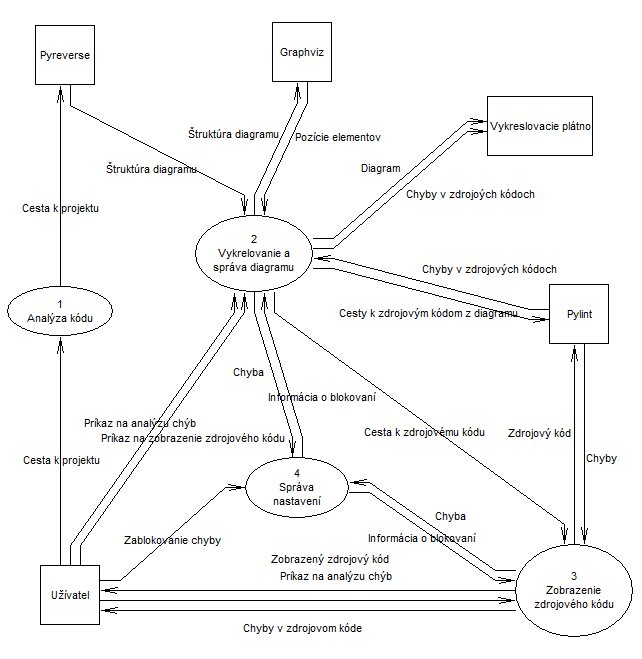
\includegraphics[width=\textwidth]{images/dfd_main}
	 \caption{DFD diagram navrhnutej aplikácie}
	\end{figure}
	
Pri spustení programu užívateľ zvolí cestu k~projektu pomocou grafického rozhrania alebo ako parameter na príkazovom riadku. Ten sa predá triede, ktorá používa metódy z~knižnice Pyreverse. Vygenerovaná štruktúra reprezentujúca diagram sa predá knižnici Graphviz~\cite{graphviz}, ktorá rozhodne o~pozíciách jednotlivých elementov diagramu tak, aby bol diagram čo najprehľadnejší. Pre každý element v~štruktúre diagramu sa vytvorí objekt knižnice Gaphas, ktorý sa vykreslí na plátne. Referencia na diagram a položky na plátne sú uložené ako kontext plátna pre neskoršie využitie. Pri spustení analýzy kódu projektu sa pomocou Pylint knižnice vygenerujú chybové hlásenia, prefiltrujú sa tak, aby sa užívateľovi nezobrazovali hlásenia, ktoré v~minulosti zablokoval. Následne pomocou kontextu plátna predajú informácie o~počte nájdených chýb a informáciách o~nich priamo jednotlivým položkám na plátne a zabezpečia ich prekreslenie. Tieto položky si uchovávajú napríklad aj informácie o~pozícii v~súbore. Po kliknutí na položku plátna sa vytvorí nové okno s~editorom podľa aktuálnych nastavení. Pri kontrole zdrojového kódu danej triedy sa pošle požiadavka danému editoru, ktorý sa stará o~zobrazovanie chýb.

	
	\section{Aplikácia jednotlivých nástrojov}
	Pre požiadavky aplikácie sme potrebovali vytvoriť triedy využívajúce alebo upravujúce funkcionalitu jednotlivých nástrojov. V~nasledujúcej podkapitole popíšeme využitie jednotlivých knižníc a ich implementáciu v~našom projekte.
	
		\subsection{Aplikácia nástroja Pyreverse}	
			Pri popise nástroja Pyreverse sme poukázali na hlavnú kostru programu Pyreverse, ktorá vracia diagram tried, predávaný triede zodpovednej za zápis. Vytvorili sme teda triedu \texttt{ScannerCommand}, ktorá spúšťa kostru programu Pyreverse v~samostatnom vlákne, prefiltruje výsledky pre potreby aplikácie a výsledky predá zapisujúcej triede, ktorú naimplementujeme.
			
			Triedu zodpovednú za zápis na plátno sme nazvali \texttt{CanvasWriter}. Táto trieda  implementuje metódu \texttt{get\_values(self, obj)}, ktorá rozhoduje, aké informácie budú predané jednotlivýcm položkám na plátne. V~tejto metóde teda rozhodneme, ktoré údaje od programu Pyreverse predáme k~ďalšiemu spracovaniu. Inak len deleguje funkcionalitu na triedu \texttt{CanvasBackend}.
		
			Trieda \texttt{CanvasBackend} rozširuje triedu \texttt{DotBackend} z~programu Pylint. Všetky výstupy tak generuje do dot~\cite{dotformat} formátu, ktoré v~prekrytej metóde \texttt{generate(self, filename)} použijeme ako vstup pre knižnicu Gaphas. 
			
			Vďaka nej dostaneme pozície jednotlivých elementov na plátne tak, aby bol výsledný graf prehľadný a uložíme potrebné informácie do kontextu plátna. Daný graf následne vykreslíme na plátno.
	

	\begin{figure}[htb]
	 \centering
	 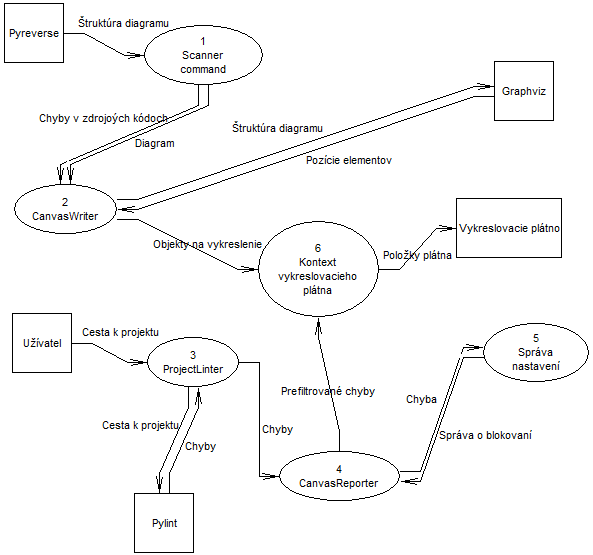
\includegraphics[width=\textwidth]{images/dfd_diagram}
	 \caption{DFD diagram procesu vykresľovania a správy diagramu}
	\end{figure}

	
		\subsection{Aplikácia nástroja Pylint}

		Nástroj Pylint využívame dvomi rôznymi spôsobmi. Potrebujeme jednak preskenovať celý projekt, aby sme chyby pre jednotlivé triedy vykreslili na plátno a zároveň potrebujeme preskenovať práve otvorený súbor. Pre každý tento účel vytvoríme triedy implementujúce funkcionalitu triedy \texttt{PyLinter} pomocou kompozície, ktoré budú bežať v~samostnatnom vlákne. 
		
		Pri kontrole samostatného súboru funkcionalitu analýzy chýb rieši každý editor samostatne. V~nasledujúcom odseku popíšeme spôsob, akým túto funkcionalitu implementuje grafický editor využívajúci komponentu GtkSourceView~\cite{gtksourceview}. Ten vytvorí inštanciu triedy \texttt{TextBufferLinter}, ktorú sme naimplementovali tak, aby jednotlivým triedam kontrolujúcim kód predala obsah textového bufferu, ktorý obdržala pri inicializácii. Nakoľko každá inštancia triedy \texttt{PyLinter} potrebuje triedu zodpovednú za výstup výsledkov, naimplementovali sme triedu \texttt{EditorReporter}.
		
		Trieda \texttt{EditorReporter} po obdržaní chybovej správy skontroluje, či nie je užívateľom blokovaná. Ak blokovaná nie je, vykreslí chybu v~zdrojovom kóde.

	
	\begin{figure}[htb]
	 \centering
	 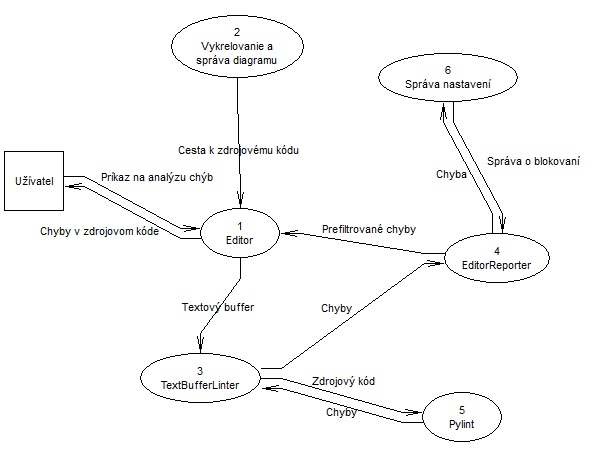
\includegraphics[width=\textwidth]{images/dfd_editor}
	 \caption{DFD diagram procesu zobrazenia zdrojového kódu}
	\end{figure}

		
	Pri kontrole celého projektu sa vytvorí inštancia triedy \texttt{ProjectLinter}, ktorej sme nastavili triedu \texttt{CanvasReporter} ako triedu zodpovednú za výstup. Trieda \texttt{CanvasReporter} pri obdržaní správy skontroluje, či nie je blokovaná a následne ju nastaví jednotlivým položkám na plátne.
 
		\subsection{Aplikácia nástroja Gaphas}
		
		Nástroj Gaphas použijeme na vykresľovanie diagramu tried na plátno. Jeho jedinou nevýhodou je prítomnosť len základných elementov ako je úsečka, obdĺžnik alebo text. Vďaka výbornému návrhu knižnice Gaphas ich ale môžeme využiť na zostavenie vlastných elementov. Z~triedy \texttt{gaphas.item.Element} odvodíme triedu \texttt{Box}, ktorá bude reprezentovať triedu. Bude taktiež uchovávať informácie o~triede, ktorú reprezentuje, ako je cesta k~súboru, názov, číslo riadku jej výskytu ale aj informácie o~chybách, ktoré detekujeme.
		
		Vzťahy medzi triedami vykreslíme za pomoci triedy \texttt{AssociationLine}, ktorá spája dve triedy \texttt{Box}. Podľa vzťahu medzi jednotlivými triedami vykreslí vzor typický pre špecializáciu alebo kompozíciu.
		
		Jednotlivé komponenty reprezentujúce triedy môžeme po plátne presúvať. Z~tohto dôvodu sme boli nútení vytvoriť obmedzenie, ktoré bude udržiavať asociačnú čiaru medzi danými dvomi triedami. Triedu sme nazvali \texttt{HandlesConstraint}. Pri pohybe komponentu si parametricky vyjadrí úsečku medzi stredmi spájaných objektov a nájde prieniky medzi ich hranami. Na dané prieniky umiestni konce spájanej úsečky.
		
		Nakoľko chceme vytvoriť rozhranie čo najviac interaktívne, potrebujeme nástroj, ktorý po dvojkliku na položku plátna zobrazí jej zdrojový kód v~nastavenom editore.
		
		Knižnica Gaphas ponúka výborné rozhranie pre tvorbu vlastného nástroja. Nástroj \texttt{OpenEditorTool} odvodíme od triedy \texttt{gaphas.tool.Tool} a v~metóde \texttt{on\_double\_click(self, event)} pristúpime k~vykreslenej položke na plátne, nad ktorou je umiestnená myš. Z~jej atribútov zistíme cestu k~zdrojovému kódu a kód zobrazíme.

		\subsection{Aplikácia ostatných nástrojov}
		
	Pre potreby aplikácie potrebujeme využiť nasledujúce nástroje:
	
				\begin{list}{•}{}
					\item ConfigParser
					\item cPickle
					\item argparse
    			\end{list}
	
	 Pre uloženie nastavení použijeme triedu ConfigParser~\cite{configparser}, ktorá umožňuje bezproblémovú prácu s~nastaveniami. Jej správanie sme pre aplikáciu prispôsobili vytvorením manažérov nastavení, ktoré implementujeme pomocou \texttt{singleton} návrhového vzoru. Takýmto spôsobom implementujeme nastavenia blokovania Pylint chýb, nastavenie použitého editora alebo uchovanie naposledy otvoreného projektu.
	
	Vlastnosťou nášho nástroja je aj ignorovanie konkrétnych chýb na jednotlivých riadkoch, ktoré ale nechceme ignorovať globálne. Informácie o~nich teda uložíme do datového kontajneru, ktorý pomocou nástroja cPickle~\cite{cpickle} serializujeme. Pri opätovnom spustení aplikácie prevedieme deserializáciu. Deserializovaný objekt neskôr použijeme na prefiltrovanie chybových správ.
	
		Module argparse~\cite{argparse} použijeme na získanie informácií, ktoré užívateľ zadá na príkazovom riadku. Modul poskytuje veľmi jednoduché rozhranie na prácu s~parametrami príkazového riadku, ako je napríklad automatická generácia nápovedy. Pomocou príkazového riadku bude môcť užívateľ zadať napríklad cestu k~projektu, ktorý sa má otvoriť, alebo typ použitého editoru.
				
\chapter{Záver}

	Našou úlohou bolo analyzovať nástroje na analýzu a vizualizáciu Python kódu a vytvoriť nástroj, ktorý poskytuje funkcionalitu, ktorú doteraz vytvorené nástroje neposkytujú.
	
	Po predstavení základných vlastností jazyka Python sme preskúmali vlastnosti jeho introspekcie, ktoré nám vytvorili prehľad o~možnosti preskúmať vlastnosti jednotlivých objektov.
	
	Neskôr sme si predstavili nástroje na analýzu kódu PEP8~\cite{pep8}, PyChecker~\cite{pychecker} a Pylint~\cite{pylint} a zhodnotili sme, že najvhodnejší nástroj pre backend našej aplikácie je program Pylint, nakoľko je ľahko prispôsobiteľný a okrem detekcie chýb poskytuje funcionalitu vygenerovania grafu. Navyše je široko používaný či už ako samostatná utilita, alebo implementáciou do~rôznych IDE modulov.
	
	Analyzovali sme taktiež existujúce nástroje na vizualizáciu kódu a zhodnotili sme ich či už po stránke funkcionality, kompaktnosti, alebo iných kritérií.
	
	Nakoniec sme preskúmali a vybrali nástroje, ktoré nám pomohli k~ľahšej implementácii projektu a projekt sme navrhli a implementovali.
	\section{Popis implementovaného nástroja}
	Implementovaný program nám umožnuje zobraziť ľubovoľný Python projekt v~podobe UML diagramu.  Výsledný UML diagram sa výzorovo podobá na diagram vygenerovaný programom Graphviz~\cite{graphviz}, no poskytuje nám okrem iného interaktívnosť a možnosť zobraziť chyby v~rámci hierarchie modulov a tried. Pomocou nastavení máme možnosť ignorovať či už celé skupiny chýb, konkrétne typy chýb, či ignorovať chyby len na konkrétnych riadkoch. Zdrojové kódy môžeme upravovať v~jednoduchých editoroch vizuálneho alebo konzolového charakteru. Aj vďaka zvoleniu vhodných knižníc program veľmi dobre škáluje a je spustený a inicializovaný za krátky čas.
	
	Medzi nevýhody programu môžeme zaradiť fakt, že slúži na analýzu len jedného programovacieho jazyka, alebo fakt, že niektorá funkcionalita, ako je napríklad filtrácia chýb, by mohla byť implementovaná na nižšej úrovni, aby bola prístupná aj spustením z~príkazového riadku bez spustenia grafického rozhrania.
	
	V~budúcnosti sa program bude môcť spustiť na iných operačných systémoch, medzi ktoré patrí napríklad aj Microsoft Windows. Ďalej bude možné viac prispôsobiť program pre jednoduchšie editovanie zdrojových kódov, akými sú napríklad klávesové skratky a iné vlastnosti pokročilých editorov.
	
	\begin{figure}[htb]
	 \centering
	 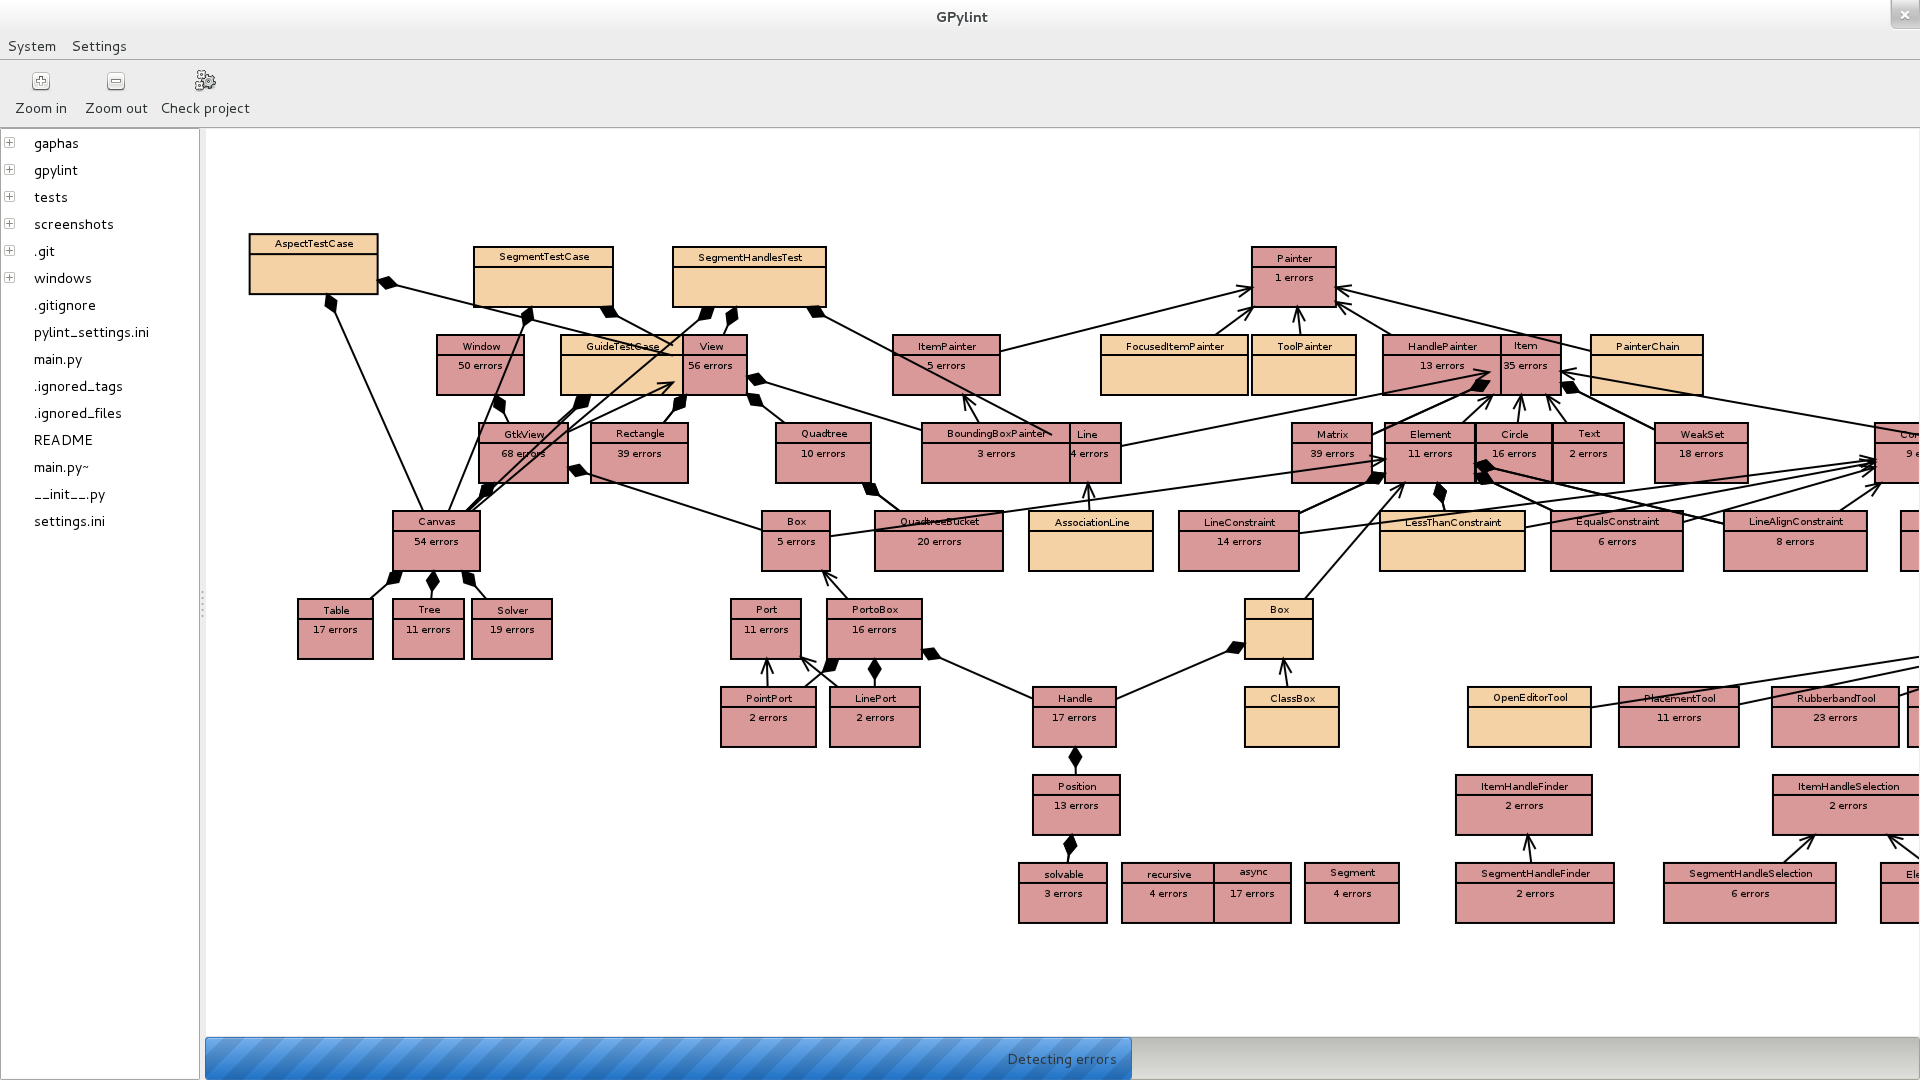
\includegraphics[width=\textwidth]{images/gpylint}
	 \caption{GPylint -- Screenshot implementovaného nástroja}
	\end{figure}
	
\begin{thebibliography}{99}

	\bibitem{pythonintro}
		\textsc{Python v2.7.3 documentation}.
		\textit{The Python Language Reference} [online].
		Apr 24, 2012 [cit. \mbox{2012-04-24}].
		Dostupný z~URL:
		\url{http://docs.python.org/reference/introduction.html}.
		
		
	\bibitem{pylint}
		\textsc{Python.org}.
		\textit{Package Index, Pylint 0.25.1} [online].
		[cit. \mbox{2012-04-24}].
		Dostupný z~URL:
		\url{http://pypi.python.org/pypi/pylint}.

	\bibitem{gaphas}
		\textsc{Python.org}.
		\textit{Package Index, Gaphas 0.7.2} [online].
		[cit. \mbox{2012-04-24}].
		Dostupný z~URL:
		\url{http://pypi.python.org/pypi/gaphas}.

	\bibitem{gtkplus}
		\textsc{Gtk.org}.
		\textit{Gtk+ website} [online].
		[cit. \mbox{2012-04-24}].
		Dostupný z~URL:
		\url{http://www.gtk.org/}.
		
	\bibitem{inspectmodule}
		\textsc{Python Software Foundation}.
		\textit{The Python Standard Library, Python Runtime Services} [online].
		Apr 24, 2012 [cit. \mbox{2012-04-24}].
		Dostupný z~URL:
		\url{http://docs.python.org/library/inspect.html}.
		
    \bibitem{pep8}
    \textsc{Python Software Foundation}.
    \textit{Python style guide checker} [online]. 1990 [cit. 12-11-2011].
    Dostupný na URL:
    \url{http://pypi.python.org/pypi/pep8/}.
    
    \bibitem{pychecker}
    \textsc{PyChecker contributors}.
    {PyChecker home page} [online].
    [cit. 12-11-2011].
    Dostupný na URL:
    \url{http://pychecker.sourceforge.net/}.
    
    \bibitem{pylint}
    \textsc{Sylvain,\,Thenault}.
    \textit{Pylint home page} [online].
    27-09-2006
    [cit. 12-11-2011]
    Dostupný na URL:~
    \url{http://www.logilab.org/project/pylint}.
    
    \bibitem{pylintfeatures}
    \textsc{PyChecker contributors}.
    \textit{Pylint features} [online].
    [cit. \mbox{2012-04-24}].
    Dostupný na URL:~
    \url{http://www.logilab.org/card/pylintfeatures}.

    \bibitem{lgpl}
    \textsc{Free Software Foundation, Inc.}.
    \textit{GNU Lesser General Public License} [online].
    [cit. \mbox{2012-04-24}].
    Dostupný na URL:~
    \url{http://www.gnu.org/copyleft/lesser.html}.   

    \bibitem{gnugpl}
    \textsc{Free Software Foundation, Inc.}.
    \textit{Gnu General Public Licence} [online].
    Dostupný na URL:~
    \url{http://www.gnu.org/licenses/gpl-2.0.html}.   

    \bibitem{pep8program}
    \textsc{Guido van Rossum,\,Barry Warsaw}.
    \textit{Style Guide for Python Code} [online].
    05-07-2001
    [cit. 12-11-2011]
    Dostupný na URL:~
    \url{http://www.python.org/dev/peps/pep-0008/}. 
        

    \bibitem{graphviz}
    \textsc{Graphviz Contributors}.
    \textit{Graphviz - Graph Visualization Software} [online].
    [cit. 12-11-2011]
    Dostupný na URL:~
    \url{http://www.graphviz.org}.    
                
        
    \bibitem{dotformat}
    \textsc{Graphviz Contributors}.
    \textit{The DOT Language} [online].
    [cit. 12-11-2011]
    Dostupný na URL:~
    \url{http://www.graphviz.org/content/dot-language}.    
        
    \bibitem{gtksourceview}
    \textsc{The GtkSourceView Team}.
    \textit{Gnome.org} [online].
    [cit. \mbox{2012-04-24}].
    Dostupný na URL:~
    \url{http://projects.gnome.org/gtksourceview/}.    
        
    \bibitem{configparser}
    \textsc{Python Software Foundation}.
	\textit{Configuration file parser} [online].
    [cit. 12-11-2011]
    Dostupný na URL:~
    \url{http://docs.python.org/library/configparser.html}.    
        
    \bibitem{cpickle}
    \textsc{Python Software Foundation}.
    \textit{Python object serialization} [online].
    [cit. 12-11-2011]
    Dostupný na URL:~
    \url{http://docs.python.org/library/pickle.html#module-cPickle}.    
    
    \bibitem{argparse}
    \textsc{Python Software Foundation}.
    \textit{Parser for command-line options, arguments and sub-commands} [online].
    [cit. 12-11-2011]
    Dostupný na URL:~
    \url{http://docs.python.org/library/argparse.html#module-argparse}.  

    \bibitem{abc}
    \textsc{Wikipedia contributors}.
    \textit{ABC (programming language)} [online].
    [cit. 12-11-2011]
    Dostupný na URL:~
    \url{http://en.wikipedia.org/wiki/ABC_%28programming_language%29}.

	\bibitem{moap}
    \textsc{MOAP contributors}.
    \textit{MOAP - Maintenance of a Project} [online].
    [cit. 12-11-2011]
    Dostupný na URL:~
    \url{http://thomas.apestaart.org/moap/trac/}.

	\bibitem{pydev}
    \textsc{PyDev contributors}.
    \textit{PyDev project} [online].
    [cit. 12-11-2011]
    Dostupný na URL:~
    \url{http://http://pydev.org/}.
	
\end{thebibliography}

\appendix
\chapter{Screenshot grafického rozhrania}

	\begin{figure}[htb]
	 \centering
	 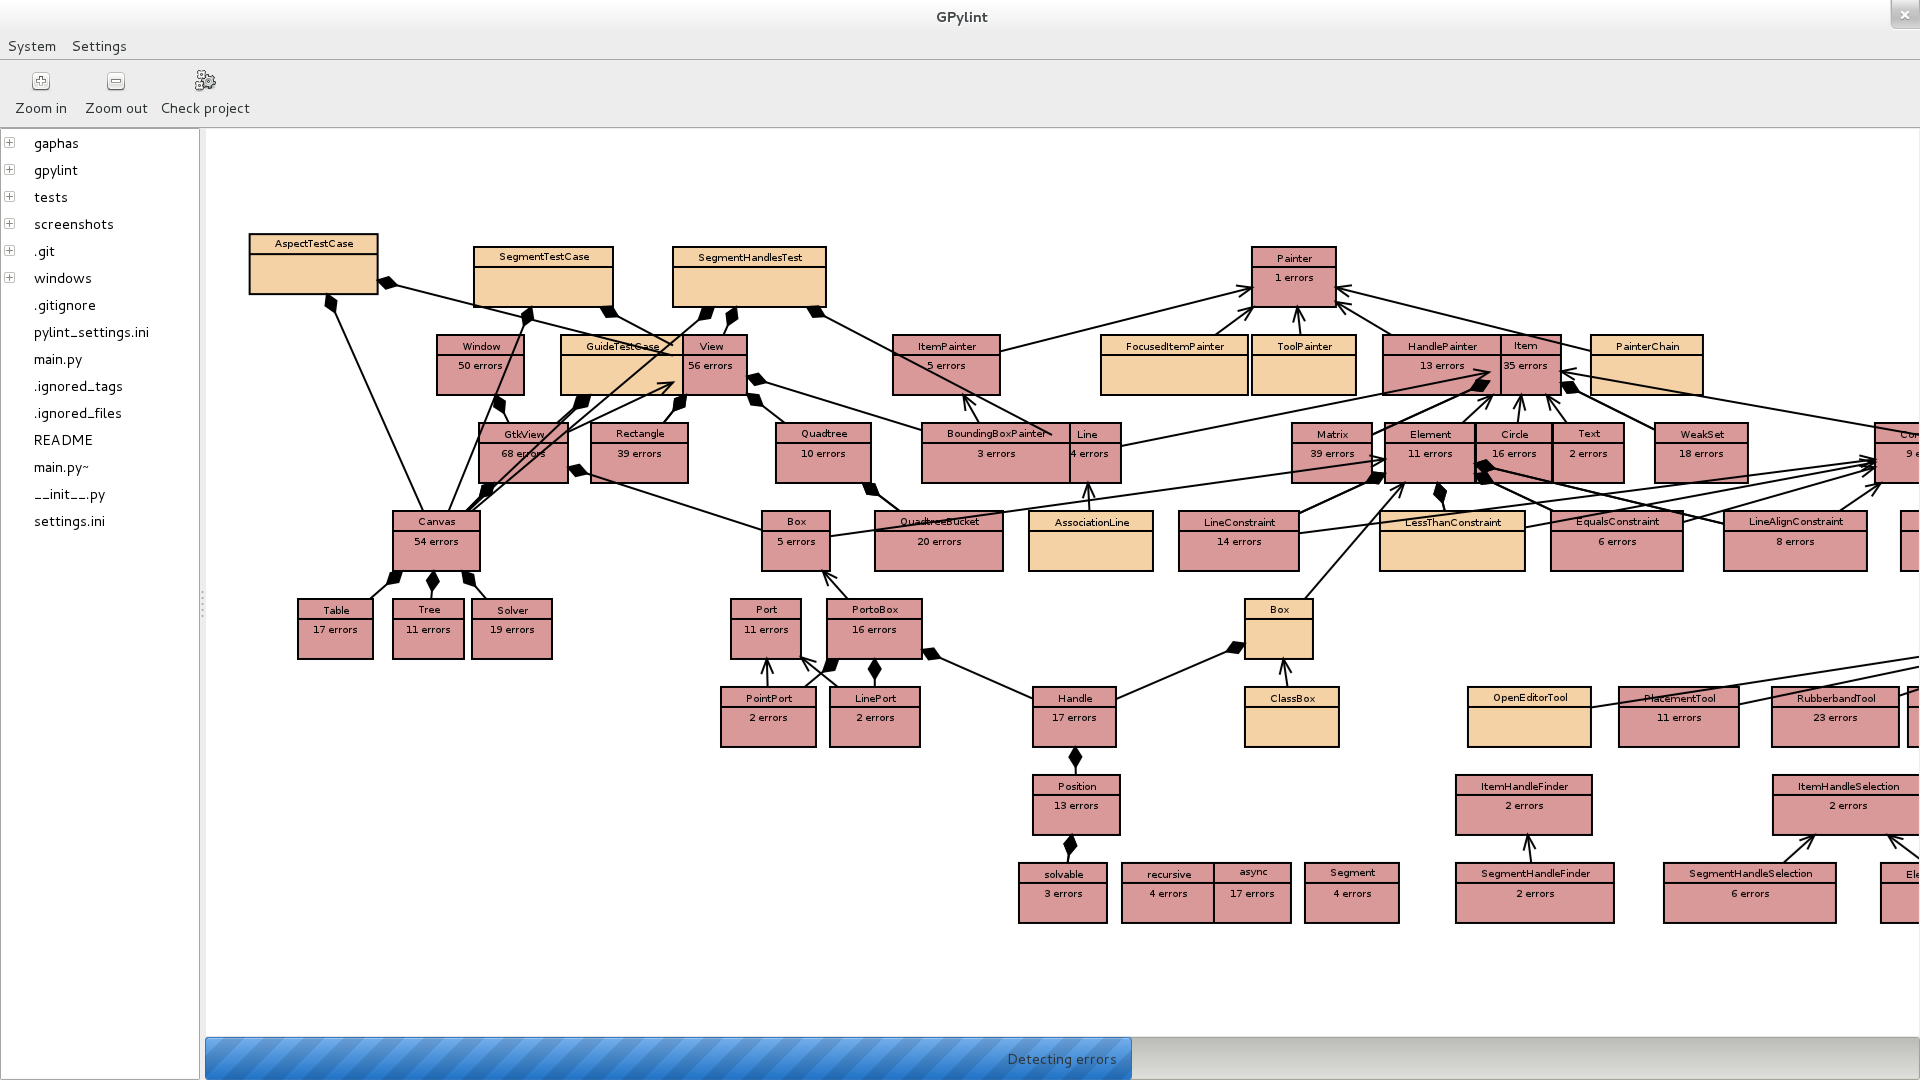
\includegraphics[width=\textwidth]{images/gpylint}
	 \caption{Diagram projektu spolu s knižnicou Gaphas zobrazený na vykresľovacom plátne počas detekcie chýb}
	\end{figure}

	\begin{figure}[htb]
	 \centering
	 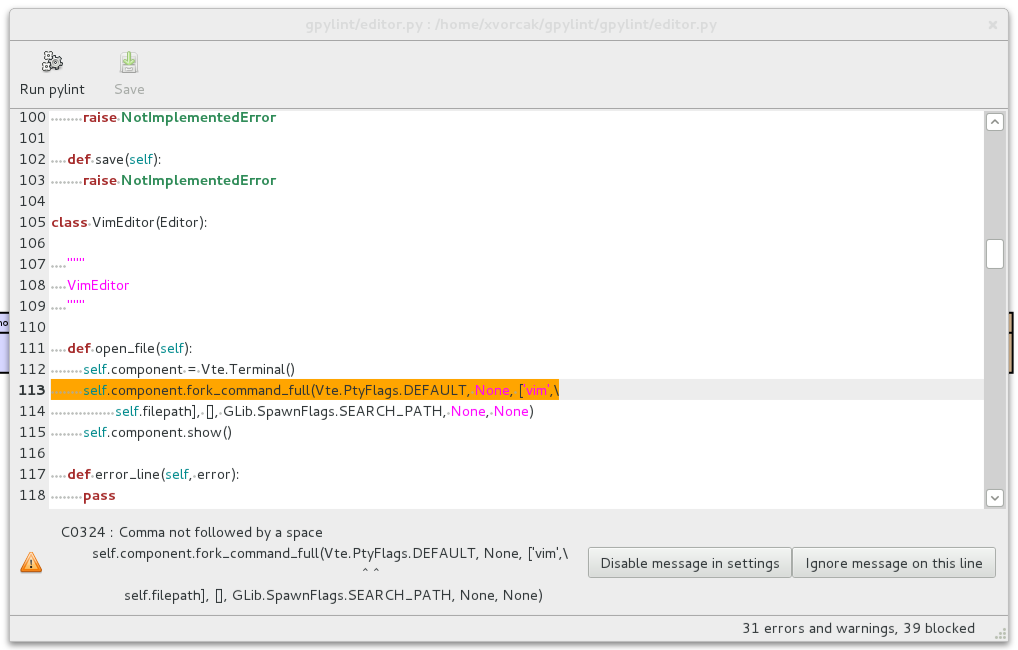
\includegraphics[width=\textwidth]{images/code_window}
	 \caption{Zobrazenie zdrojového kódu vo vizuálnom editore}
	\end{figure}
			    
	\begin{figure}[htb]
	 \centering
	 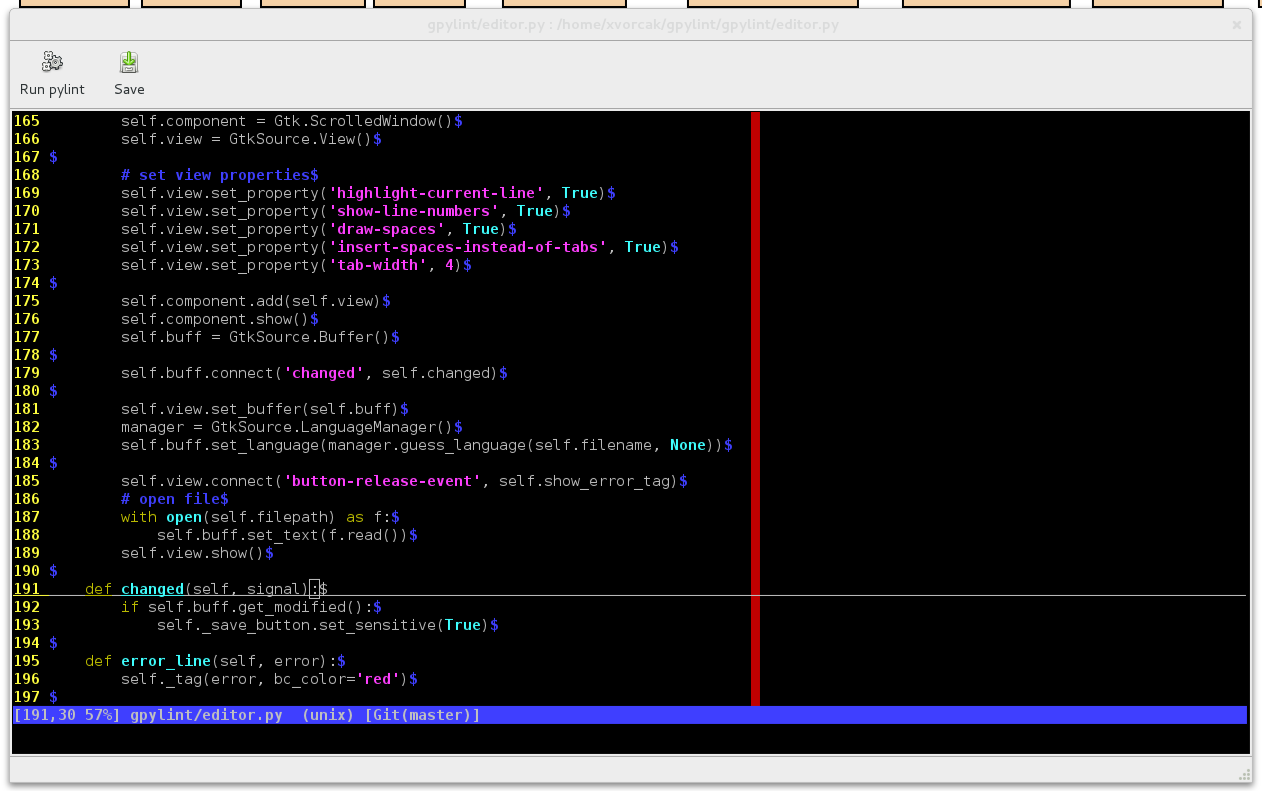
\includegraphics[width=\textwidth]{images/vim_editor}
	 \caption{Zobrazenie zdrojového kódu v editore Vim}
	\end{figure}
	
	\begin{figure}[htb]
	 \centering
	 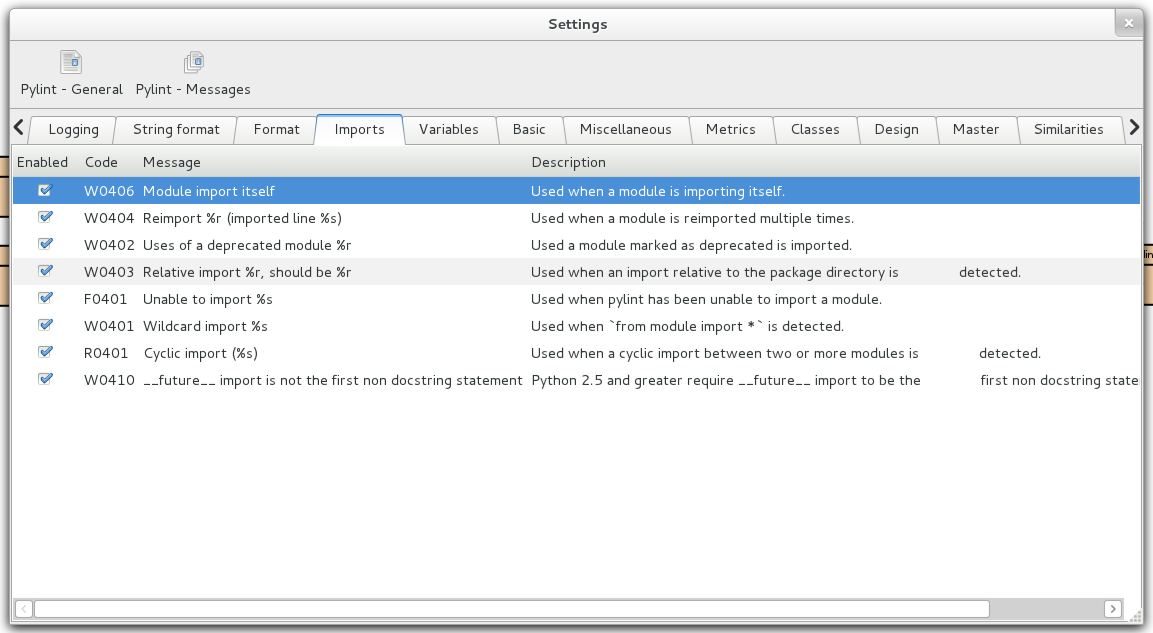
\includegraphics[width=\textwidth]{images/settings}
	 \caption{Okno nastavení chybových hlášok}
	\end{figure}
		
\chapter{Obsah priloženého CD}

\begin{itemize}
\item Aplikácia GPylint

	\begin{itemize}
	 \item \emph{gpylint} -- zložka obsahujúca Git repozitár programu
	 \item \emph{logilab.patch} -- patch, ktorý odstraňuje bug balíčku logilab.astng.inspector, \url{http://www.logilab.org/ticket/92362}
	 \item \emph{gpylint/README} -- súbor obsahujúci základné informácie pre beh programu
	\end{itemize}



\item Text bakalárskej práce

	\begin{itemize}
	 \item \emph{thesis.tex} -- text bakalárskej práce vo formáte latex s využitím šablóny fithesis
	 \item \emph{thesis.pdf} -- text bakalárskej práce vo formáte PDF
	 \item \emph{images} -- zložka obsahujúca obrázky použité v bakalárskej práci
	 \item \emph{fithesis2.cls} -- šablóna fithesis2
	\end{itemize}
	
\end{itemize}

\end{document}
